\documentclass[french]{article}
\usepackage[utf8]{inputenc}
\usepackage[french]{babel}
\usepackage[T1]{fontenc}
\usepackage{graphicx}
\graphicspath{ {./} }
\usepackage{listings}
\usepackage{xcolor}
\usepackage{float}
\usepackage{hyperref}
\hypersetup{
    colorlinks,
    linkcolor={black!50!black},
    citecolor={blue!50!black},
    urlcolor={blue!80!black}
}

\definecolor{background}{RGB}{248, 249, 250}
\definecolor{border}{RGB}{234, 236, 240}
\definecolor{foreground}{RGB}{36, 41, 46}
\definecolor{comments}{RGB}{106, 115, 125}
\definecolor{string}{RGB}{0, 92, 197}
\definecolor{keywords}{RGB}{176, 0, 70}

\lstdefinestyle{mystyle}{
    backgroundcolor=\color{background},   
    commentstyle=\color{comments},
    keywordstyle=\color{keywords},
    numberstyle=\tiny\color{foreground},
    stringstyle=\color{string},
    basicstyle=\ttfamily\footnotesize,
    breakatwhitespace=false,         
    breaklines=true,                 
    captionpos=b,                    
    keepspaces=true,                 
    numbers=left,                    
    numbersep=5pt,                  
    showspaces=false,                
    showstringspaces=false,
    showtabs=false,
    frame=single,
    rulecolor=\color{border},
    tabsize=2
}

\lstset{style=mystyle}


\title{\textsc{ - PROJET S6 -} \\ Tower Defense \\ \textsc{ - } }
\author{Mathias ROSA, Mohamed REKIK,\\ Mathias APARICIO, Hugo BASTIEN}
\date{mai 2023}

\begin{document}


\maketitle
\vspace{10cm}
\begin{figure}[ht]
    \centering
    
\includegraphics[width=0.5\textwidth]{logo_emmk.jpg}
    \label{fig:logo_emmk}
\end{figure}

\newpage

\tableofcontents

\newpage
\section{Introduction}
Ce projet se situe dans l'UE projets du semestre 6 et nous offre l'opportunité d'appliquer les enseignements reçus en cours de  programmation fonctionnelle. La durée était de 6 semaines répartis en séances de 4h20 les mardi après-midi.
Afin de créer une base de code plus robuste, une vérification de types est appliquée en utilisant le compilateur tsc et en écrivant le code en TypeScript.

Pendant les séances, nous avons été aidés par \textbf{Vinh-Thong TA} que nous remercions chaleureusement.
%\newpage
\section{Le projet Tower Defense}


\subsection{Présentation du sujet}

% description du projet

Le sujet du projet est le jeu du tower Defense. C'est un jeu de vidéo, où une horde de monstre défile vers un point d'arrivée, si un monstre atteint le point d'arrivée le joueur a perdu. Le joueur peut empêcher les monstres d'atteindre ce point en plaçant des tours autour du chemin. 
Si le joueur arrive à tuer tous les monstres sans perdre avant, il gagne. Un bonus était octroyé si on arrivait à garder le même principe du jeu, mais sans violence.

Le but de ce projet est d'appliquer les notions vues pendant le cours de programmation fonctionnelle comme la pureté et la citoyenneté de première classe en développant un jeu de type Tower Defense.
Pour ce projet, l'utilisateur doit pouvoir lancer des parties qui seront automatiques : il n'a pas à interagir dessus.

\subsection{Réalisations}

% Ce qu'on a fait
% Parler de TypeScript ?

Dans notre Tower Defense, il existe trois types d'acteurs : Les Spawners, les Tours et les Gobelins. Ils interagissent sur un monde.
Le monde est composé d'un ensemble de cases de types différents. Il existe des chemins qui relient les éventuelles multiples cases de départ et d'arrivée, des cases constructibles et des cases non constructibles contenant par exemple des arbres ou des rochers.
La partie se déroule en un ensemble de phases. Il existe par exemple une phase "move" pendant laquelle bougent les acteurs pouvant se déplacer ou encore une phase "attaque" assez explicite.

Au début de la partie, le monde ne contient que des Spawners. Le rôle des Spawners est de créer des acteurs au long de la partie. Ils sont placés sur les cases conductibles étant à proximité d'un chemin et sur les cases de départ.
Les Tours sont considérées comme faisant partie de la défense et les gobelins faisant partie de l'attaque.

On peut suivre le déroulement de la partie en mode terminal ou en utilisant l'interface WEB présentée figure \ref{fig:visualisation}.

\begin{figure}[H]
    \centering
    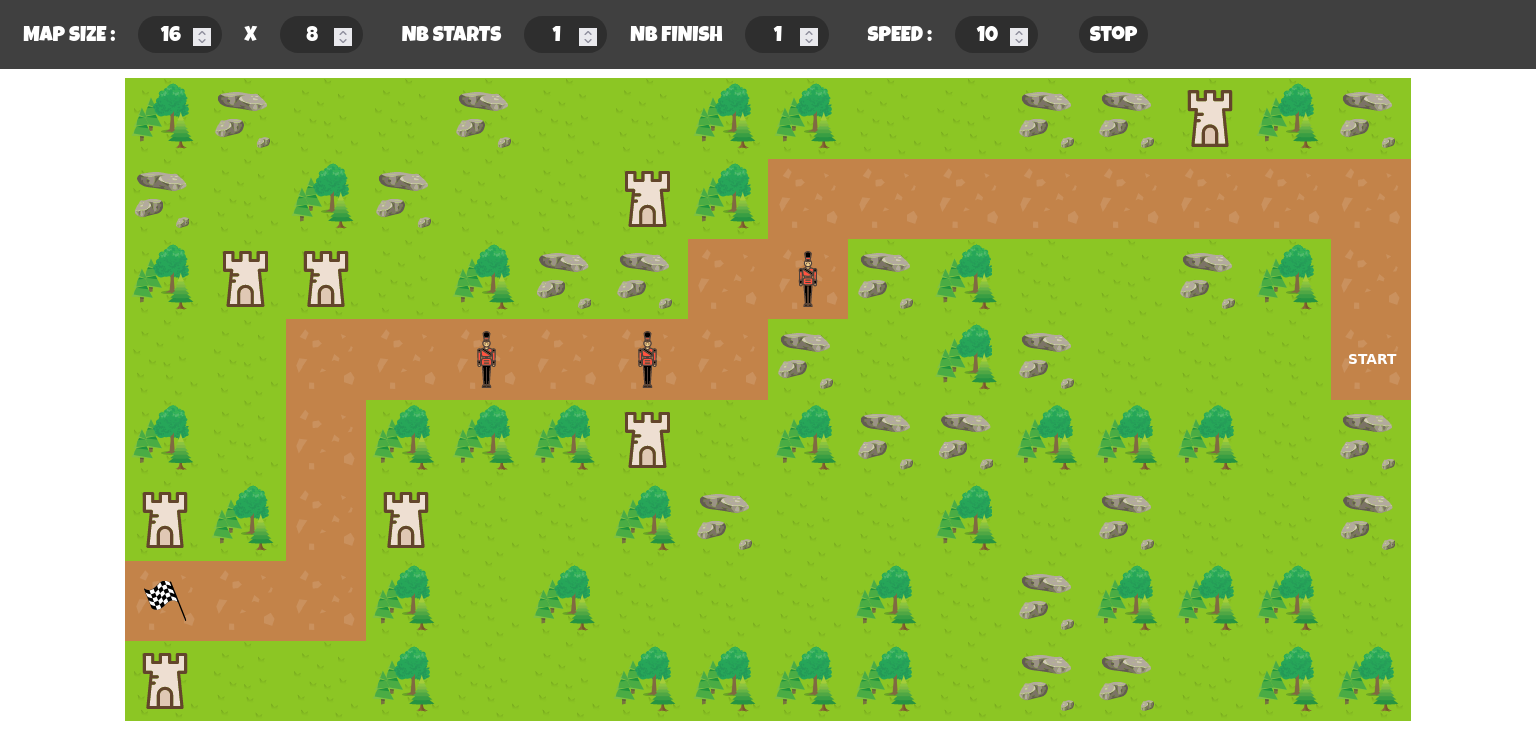
\includegraphics[width=\textwidth]{TowerDefense.png}
    \caption{Visualisation WEB d'une partie}
    \label{fig:visualisation}
\end{figure}
Sur le client graphique on peut modifier la taille de la map, le nombre de cases de départs pour les "gobelins" le nombre de cases d'arrivées et enfin le temps entre chaque tour du jeu. Ce dernier paramètre s'est avéré très utile pendant la phase de débogage, en effet grâce à l'historique présent dans la console lancer des parties avec un temps ralenti a permis de mettre en lumière des bugs qui aurait été plus dur a tracé avec une vitesse de jeu constante. 
\subsection{Organisation du projet en modules}

% Comment on l'a fait : 
% - description des fichiers, leurs role
% - description des types ? autre partie ?

Ce projet est organisé en plusieurs sous dossiers.
\begin{itemize}
    \item Le dossier \textbf{src} contient les fichiers sources en TypeScript et le fichier index.html servant de base pour l'affichage.
    \item Le dossier \textbf{tst} contient les descriptions des tests.
    \item Le dossier \textbf{public} contient les ressources nécessaires à la génération de l'interface WEB comme les styles et les images.
\end{itemize}


Voici figure \ref{fig:graph} le graphe des dépendances entre les modules de ce projet.

\begin{figure}[H]
    \centering
    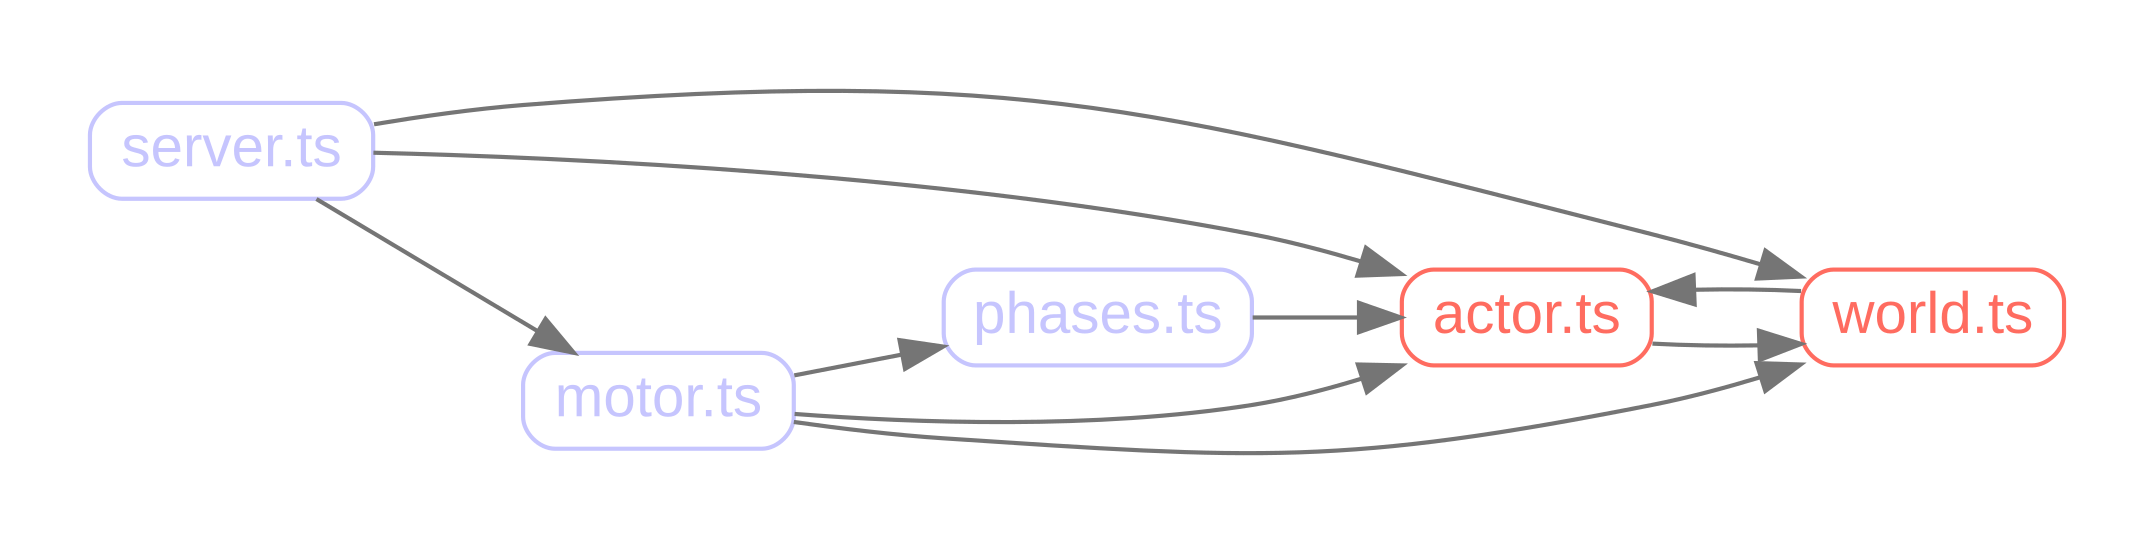
\includegraphics[width=\textwidth]{graph.png}
    \caption{Graphe des dépendances entre les modules}
    \label{fig:graph}
\end{figure}



% On décrit le fonctionnement des fichiers

Après étude du sujet, nous avons décidé de diviser le projet en plusieurs modules ayant chacun un rôle défini.
La structure du monde est définie dans \textbf{world.ts}, les acteurs et leurs interactions sont définies dans \textbf{actor.ts}, les phases de jeu dans \textbf{phases.ts}.
Ces modules interagissent entre eux grâce à un moteur de jeu que l'on peut retrouver dans \textbf{motor.ts}.
L'interface utilisateur est gérée depuis \textbf{server.ts} qui génère les éléments dans la page HTML.

\subsubsection{Architecture du monde}

Nous avons décidé de représenter le monde comme une grille de places. Une place possède un type parmi "road", "land", "rocks", "tree", "start", "finish" et "edge".
Les places "road" relient les "start", d'où partent les acteurs et les "finish".
Les places "land" sont constructibles, des tours peuvent  donc y apparaître en cours de partie.
Les autres places composent le reste du monde, servent surtout de décors et ne sont pas constructibles.
Le monde est généré procéduralement lors de son initialisation et est ensuite immuable.
Pour s'inscrire dans une démarche de programmation fonctionnelle et pour profiter des possibilités offertes par un langage de haut niveau comme TypeScript, la génération du monde a été décomposée en plusieurs étapes chacune étant réalisée par une fonction renvoyant un monde.changement
Dans la version actuelle du projet, on commence par générer un monde ne contenant des "land", "tree" et des "rocks".
À ce monde, on rajoute autant de cases de départ que l'on souhaite. Pour ce faire, il suffit de réappliquer la fonction qui ajoute une case de départ autant de fois qu'on souhaite avoir de cases de départ. On fait de même pour les cases de d'arrivée. On rajoute ensuite un chemin et notre monde est généré.
Cette méthode de génération est généralement plus coûteuse qu'une version impérative, car elle implique de recréer un nouveau monde à chaque fois, mais elle nous permet de créer des mondes assez différents très facilement.
Cette méthode nous permettrait également de modifier très simplement la génération du monde pour rajouter par exemple un type de place rivière ou encore volcan et ainsi imaginer de nouvelles parties.
Pour pouvoir interagir avec ce monde, de nombreuses fonctions ont étés créés.
Celles-ci sont toutes pures afin de pouvoir facilement être composées et testées. Elles ont étés conçus afin de minimiser un éventuel changement de d'implémentation pour certaines structures du code à un moment donné.

\begin{figure}[H]
    \centering
    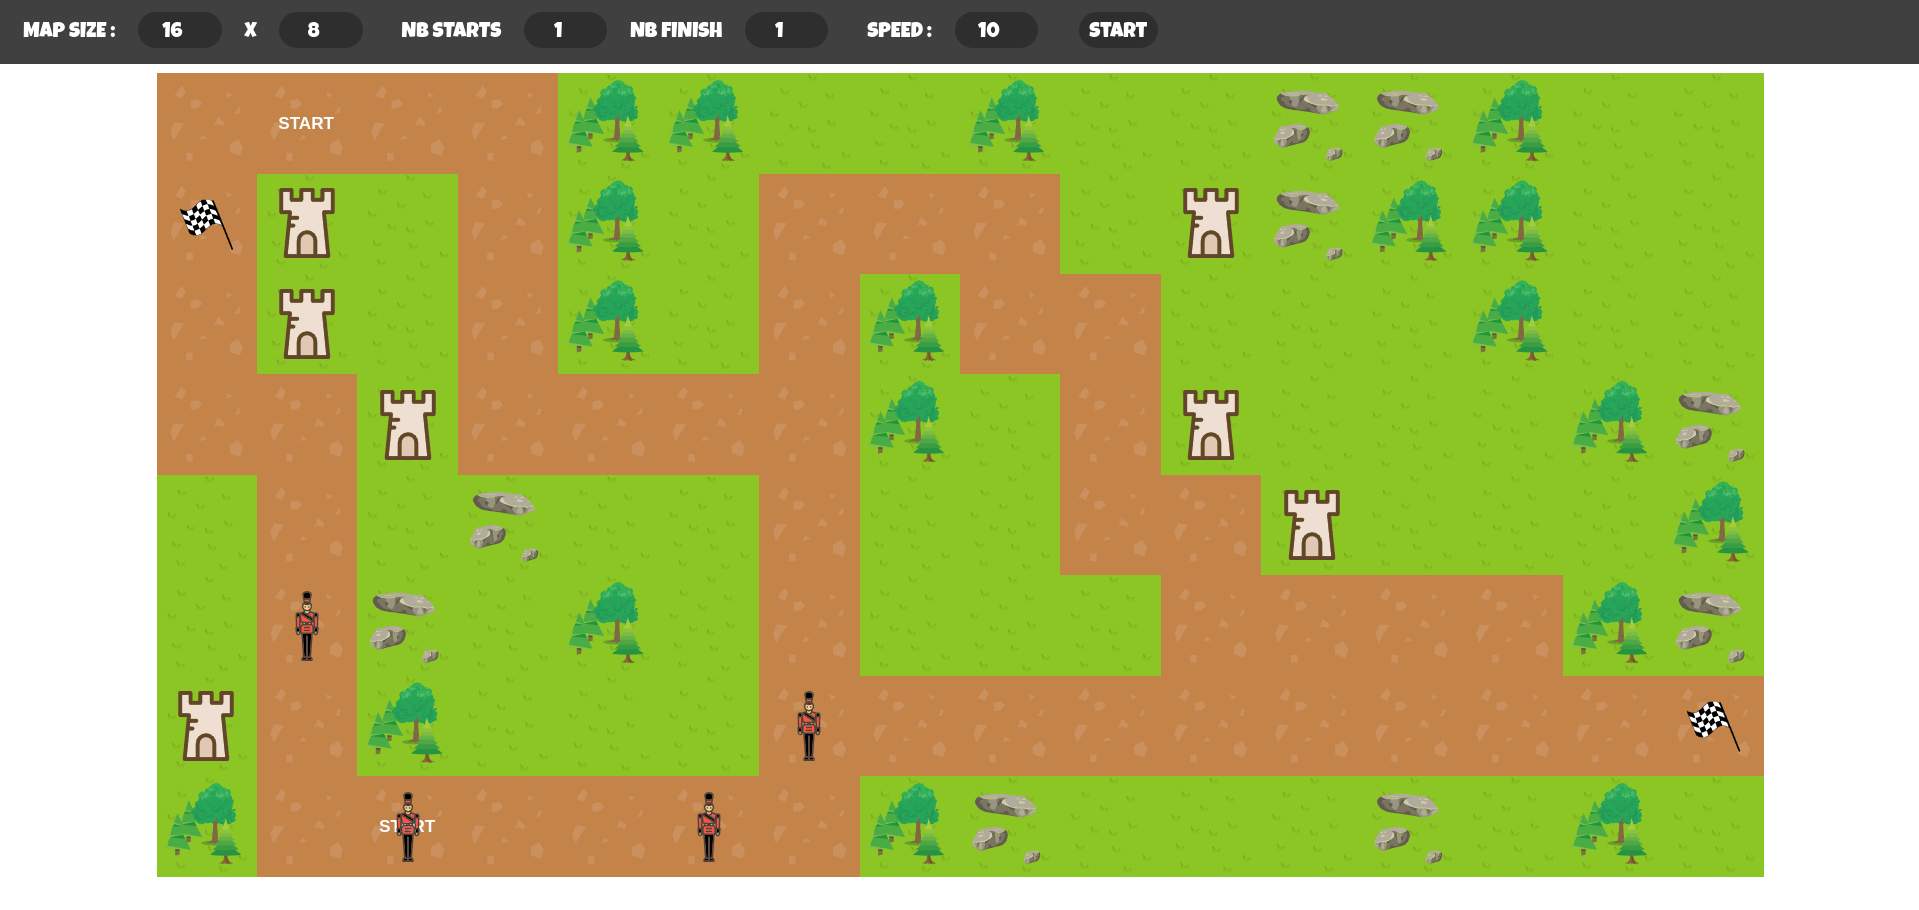
\includegraphics[width=\textwidth]{plusieurs_starts_ends.png}
    \caption{Visualisation WEB d’une partie avec deux cases de départs et deux cases d'arrivées}
    \label{fig:graph1}
\end{figure}



\subsubsection{Les acteurs}

Nous avons décidé de décrire les acteurs comme des objets ayant un identifiant, un type, une position, une vie et un ensemble d'actions.
Les acteurs seront stockés sous la forme d'un tableau d'acteurs initialisé en début de partie. Lorsqu'un acteur interagit avec le monde ou subit une interaction d'un autre acteur, il est remplacé par un nouvel acteur ayant subi les modifications nécessaires.
Afin d'agir sur le monde, chaque acteur possède un ensemble d'actions. Ces actions sont des fonctions qui prennent en paramètre le monde, l'acteur et la liste des acteurs et renvoient un acteur comportant les modifications nécessaires.
Dans le cas d'un Spawner par exemple, le nouvel acteur créé sera renvoyé par la fonction "spawn" du Spawner.
Tout comme pour la génération du monde, nous avons souhaité que les acteurs puissent être créés en composant des fonctions pures.
Cela nous permet de créer des acteurs ayant des caractéristiques variées très facilement et de les modifier très simplement.
Pour faciliter la création d'acteurs et la rendre plus modulable, nous avons créé des fonctions qui renvoient des fonctions pour les adapter.
C'est le cas de la fonction "attackActor" qui prend en argument le nombre de dommages à appliquer, le rayon d'attaque et le type d'acteur à attaquer et renvoie une fonction permettant d'attaquer un acteur avec les différents paramètres. Cela nous permet de réutiliser par exemple le code de l'attaque d'un gobelin par une tour et d'une tour par un gobelin même si les dommages à appliquer ne sont pas les mêmes.


\subsubsection{Le moteur}

Maintenant que nous avons un monde et des acteurs, il faut pouvoir les faire interagir.
Pour ce faire nous avons créé un moteur de jeu qui va appliquer les actions des acteurs sur le tableau d'acteurs.
Le moteur de jeu a lui aussi été conçu dans le paradigme fonctionnel.
La fonction principale correspond à la boucle de jeu et est modulable dans le sens où elle permet de configurer la génération du monde, de choisir la fonction à utiliser pour l'affichage ainsi que celle déterminant l'attente entre chaque tour.

La fonction déterminant l'attente entre chaque tour est une fonction asynchrone qui renvoie une promesse de chaîne de caractères. Une fois la promesse résolue, la boucle de jeu est relancée.
Cette approche nous permet d'avoir un temps d'attente dynamique pendant la partie, mais également d'interpréter des actions comme l'envoi d'un signal d'arrêt. Dans le cas où la promesse renvoyée est "stop", la boucle de jeu s'arrête, ce qui est utile pour mettre fin à des parties longues où recommencer une partie sans attendre la fin de la partie précédente, ce qui causerait des bugs sur l'affichage.

Les conditions de fin de jeu sont également définies dans une fonction séparée et donc elles peuvent être modifiées très facilement.

\subsubsection{Le serveur}

Une partie de ce projet propose de produire une visualisation WEB du jeu.
Pour générer cette visualisation, le sujet nous propose d'utiliser le bundler Parcel.
L'idée de créer un "serveur" provient d'une volonté de séparer la génération du monde et le moteur de jeu de l'interface WEB.
Le serveur aura donc la tâche d'appeler la fonction implémentant la boucle de jeu qui est incluse dans le moteur. 
Elle devra lui passer les bons paramètres afin de générer le monde avec les caractéristiques souhaitées par l'utilisateur ainsi que la fonction qui permet de générer l'affichage.
Puisqu'il gère l'affichage, il est inclus dans le fichier "index.html", ce qui lui permet d'avoir accès au DOM (Document Object Model).
Ceci lui permet de modifier le contenu de la page, ce qui est utile pour afficher le monde et les acteurs.
Pour que les utilisateurs puissent paramétrer le monde, le serveur utilise également le DOM pour écouter les événements de l'utilisateur. 

Puisqu'on souhaite que les utilisateurs puissent changer le temps d'attente entre chaque tour et envoyer un signal d'arrêt, comme expliqué dans la partie Réalisations, c'est dans le serveur que l'on va coder cette fonction. 

Lancer plusieurs jeux en même temps provoque des conflits au niveau de l'affichage, ainsi, le dernier jeu en cours est toujours stoppé avant de lancer le nouveau.
Une variable globale au module a donc été créé afin de pouvoir suivre si un jeu est en cours ou non.


\newpage
\section{Importance des Tests}


Il est important lors de l'élaboration d'un projet de tester les différentes parties du code afin de s'assurer que tout fonctionne comme prévu.

Pour un projet de programmation fonctionnelle, faire des tests est également important car, ceci permet de montrer une caractéristique supplémentaire de ce paradigme, à savoir la facilité de testabilité.
En effet, nos fonctions étant pour la plupart pures, ne dépendent pas d'un contexte et sont censées renvoyer le même résultat pour les mêmes paramètres ce qui permet de les tester très facilement.

Dans ce projet, comme proposé par le sujet, nous utilisons le module Jest afin de faire des tests.
Ce module est particulièrement adapté à la programmation fonctionnelle, car il peut facilement prendre fonction en paramètre et vérifier que le résultat est bien celui attendu.

De plus, cela nous a permis de gérer efficacement la complexité du projet, en le découpant en fonctions plus petites et plus facilement testables.

\newpage

\section{Conclusion}
La réalisation du projet Tower Defense nous a permis d'appliquer les enseignements de Mr Renault en programmation fonctionnelle. Nous avons utilisé le langage TypeScript pour développer le jeu, ce qui a garanti une plus grande exigence sur le code écrit, et nous avons structuré le projet en modules afin d'organiser le code de manière quasi indépendante et modulaire.

L'architecture du monde, la gestion des acteurs et le moteur de jeu ont été conçus en suivant les principes de programmation fonctionnelle, i.e voir les fonctions comme des briques qu'on empile pour former des objets. La pureté et l'aspect fonctionnel du projet a facilité les tests. L'utilisation de Jest a permis d'unifier la conception de test et d'avoir un affichage clair de la couverture des fonctions développé. 

La génération procédurale du monde, la création des acteurs ont été implémentées de manière pure, ce qui nous a offert une grande flexibilité pour en créer de différents types.

L'interface utilisateur, réalisée à l'aide d'une page HTML, nous a permis de visualiser le déroulement du jeu et de pouvoir changer des paramètres qui se sont avérés utiles pour le débogage notamment. 

En conclusion, ce projet nous a permis d'approfondir nos connaissances en programmation fonctionnelle et de les appliquer dans un contexte concret. Nous avons pu expérimenter l'organisation modulaire du code, la génération procédurale et la gestion des interactions entre les acteurs. Ce fut une expérience enrichissante qui nous a permis de renforcer nos compétences en développement logiciel afin de nous préparer à notre futur métier d'ingénieur.


\end{document}

